\documentclass[tikz,border=3mm]{standalone}
\usetikzlibrary{calc}
\newcommand{\equicenter}[2]
{
	\def\r{#1} % bán kính đường tròn bé nhất
	\def\a{6*#1} % bán kính đường tròn to nhất
	% #2 tọa độ tâm các đường tròn
	\foreach \i in {1,2,3,4,5,6}
	\draw[gray] #2 circle(\i*\r);
	\draw[magenta, shift={#2}] (\a,0)--(0,\a)--(-\a,0)--(0,-\a)--cycle;
} % end of \equicenter command
\begin{document}
	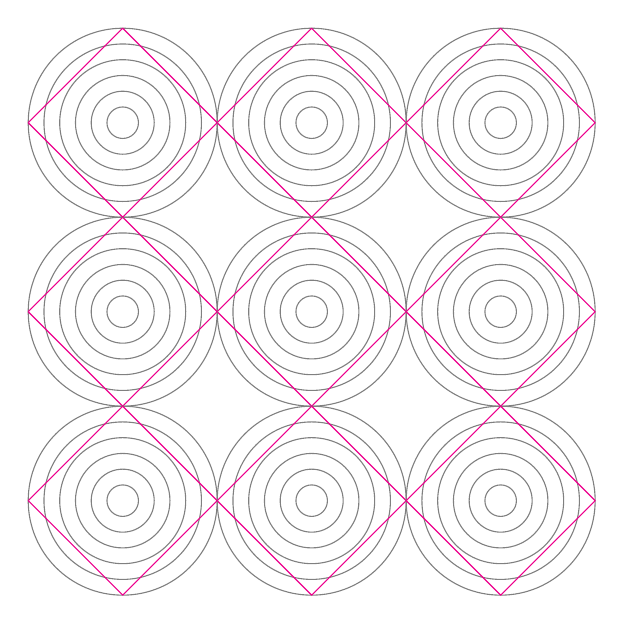
\begin{tikzpicture}[line cap=round,line join=round]
		\foreach \c in {(0,0),(2.4,0),(-2.4,0),(0,2.4),(0,-2.4),(2.4,2.4),(-2.4,-2.4),(-2.4,2.4),(2.4,-2.4)}
		\equicenter{.2}{\c};
	\end{tikzpicture}
\end{document}